\chapter{Conclusion and Future Work}

\section{Summary}

Over the past few decades, the evolution of custom hardware has seen its fair share of highs and lows. A decade ago, the idea of incorporating a custom computing device into each server within a data center was nothing short of a pipe dream. However, in recent years, the trend towards large-scale cloud computing, the demands of data center applications, and the performance limitations of general-purpose processors have accelerated the development of custom hardware. This has resulted in a significant improvement in the performance of data center networks.

The advancement of custom hardware and the communication requirements of distributed systems have led to the widespread deployment of programmable network cards in data centers. Microsoft uses FPGAs to boost the performance of search engines, virtual networks, compression, machine learning inference, and so on. Amazon and Alibaba Cloud enhance virtual networks, virtual storage, and virtual machine monitors. Tencent Cloud employs FPGAs, while Huawei Cloud utilizes network processors to speed up virtual networks. Looking back, network virtualization may have been the first major application of programmable network cards, but this only scratches the surface of the potential of these devices.

To fully leverage the high performance of data center networks, it is crucial to minimize the "data center tax". This includes not just network virtualization, but also network functions and operating system communication primitives. This paper proposes the acceleration of network functions using FPGA-based programmable network cards. To simplify FPGA programming, this paper introduces the first FPGA programming framework suitable for high-speed network packet processing based on high-level languages. This improves throughput tenfold and reduces latency to a tenth compared to traditional CPU-based network functions. To decrease the overhead of operating system communication primitives, this paper suggests a combined software-hardware user-space socket system. This system is fully compatible with existing applications and can achieve throughput and latency close to hardware limits. This resolves the longstanding conflict between the low performance of general protocol stacks and the poor compatibility of dedicated protocol stacks.

The term "programmable network card" is derived from network acceleration, but its influence extends beyond the network and continues to permeate various areas of the system. Memory data structure storage is a crucial foundational component of distributed systems. This paper introduces a remote direct key-value access primitive, an extension of the remote direct memory access (RDMA) primitive. By bypassing the server-side CPU and directly accessing the host memory with the programmable network card, along with a series of performance optimizations, this paper achieves a throughput ten times that of the CPU key-value storage system and microsecond-level latency. This makes it the first general-purpose key-value storage system with a single-machine performance reaching one billion operations per second.

Without a doubt, programmable network cards can enhance system performance and reduce data center costs. The three systems proposed in this paper establish new performance benchmarks for virtual network functions, general memory key-value storage, and socket network protocol stacks. However, the aim of this paper is not to break performance records, but to inspire readers to consider: How can we build a programmable network card ecosystem that includes hardware, development toolchains, and operating systems? How will new hardware, such as programmable network cards, alter the architecture of data centers and the programming paradigm of distributed systems? As it has been said, "The best way to predict the future is to create it". The story of programmable network cards is just beginning.

\section{Future Work}

High-performance data center systems based on programmable network cards necessitate a combined software-hardware ecosystem, primarily composed of hardware, development toolchains, and operating systems. Section \ref{future:progammable_nic} will discuss the future hardware architecture of programmable network cards. The development toolchain, including programming frameworks, compilers, runtime libraries, debugging tools, etc., is vital in software-hardware co-design. Section \ref{future:toolchain} will discuss future works in the development toolchain. The operating system, including virtualization, scheduling, monitoring, high availability, flexible scaling, etc., will be discussed in Section \ref{future:os}. Finally, as a first-class citizen in the data center, the programmable network card not only enhances system performance but also prompts us to rethink the overall architecture of distributed systems, which may lead to system innovation. This will be discussed in Section \ref{future:system}.

\subsection{Programmable Network Card Based on System-on-Chip}
\label{future:progammable_nic}

\begin{figure}[htbp]
	\centering
	\subfloat[The Catapult programmable network card used in this paper.]{
		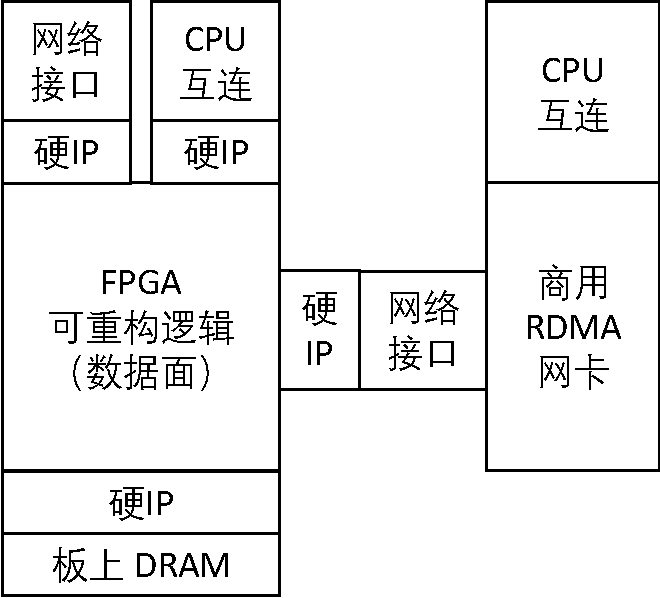
\includegraphics[width=0.4\textwidth]{figures/smartnic-current.pdf}
		\label{conclusion:fig:smartnic-current}
	}
	\hspace{0.05\textwidth}
	\subfloat[Future system-on-chip.]{
		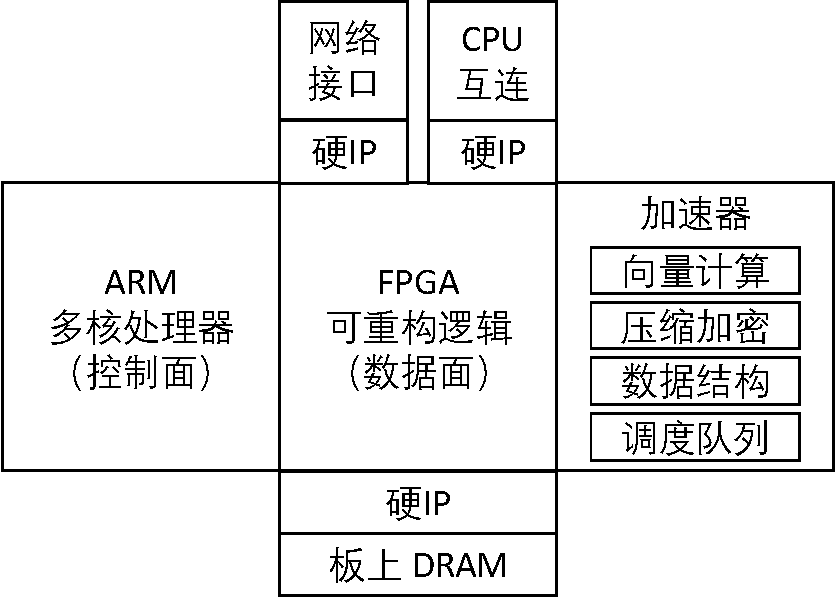
\includegraphics[width=0.5\textwidth]{figures/smartnic-soc.pdf}
		\label{conclusion:fig:smartnic-soc}
	}
	\caption{Comparison of programmable network card structures.}
\end{figure}

This paper utilizes the Catapult programmable network card depicted in Figure \ref{conclusion:fig:smartnic-current}. This architecture has three limitations. Firstly, the performance of existing commercial RDMA network cards significantly decreases when the number of concurrent connections is large \cite{mprdma}. We aim to use the scalable key-value storage technology in Chapter \ref{chapter:kvdirect} to implement the RDMA hardware transmission protocol in FPGA reconfigurable logic to achieve high performance under high concurrent connection numbers. This has been discussed in Section \ref{socksdirect:sec:discussion}. Secondly, FPGA is only suitable for accelerating the data plane, and the control plane is still left on the host CPU. Although its computing power is not large, for performance isolation, computing nodes still need to reserve a small number of CPU cores for control plane processing. Chapter \ref{chapter:intro} has pointed out that even reserving a physical CPU core is quite expensive. For this reason, we hope to add ARM multi-core processors to the programmable network card to implement the control plane, thereby completely eliminating the virtualization overhead on the host CPU. The cost of ARM multi-core processors is tens of dollars, far lower than the cost of a physical CPU core. Finally, some types of workloads are not very efficient when implemented in FPGA and should be solidified in ASIC accelerators. The first type is computationally intensive operations such as vector operations, encryption and decryption operations in deep learning and machine learning. For example, the RSA asymmetric encryption based on the Intel QuickAssist accelerator card \cite{intel-qat} is about 10 times higher in throughput than the FPGA-based implementation in Chapter \ref{chapter:clicknp}; the LZ77 compression algorithm based on ASIC is also an order of magnitude higher in throughput than the FPGA-based implementation in this paper. The power consumption, area, and process of the used ASIC and FPGA chips are close. The second type is common data structures and scheduling queues. The lookup table based on Content-Addressable Memory (CAM) is a necessary component of many common data structures such as hash tables, out-of-order execution engines, caches, fuzzy matching tables, etc. CAM can be implemented with ternary gates in ASIC, but the efficiency of implementation in FPGA is low \cite{wong2011comparing}. In addition, priority queues (which can be implemented with shift register sequences or heaps), round-robin scheduling queues, out-of-order execution schedulers considering dependency relationships, timers, and other structures are widely used in many applications, so they can learn from the architecture of network processors, harden these general structures, and let FPGA reconfigurable logic focus on customized computing and flexible interconnection.

Therefore, this paper anticipates that future programmable network cards will utilize the system-on-chip architecture as depicted in Figure \ref{conclusion:fig:smartnic-soc}. Compared to separate components interconnected by off-chip buses, the system-on-chip can offer higher bandwidth and lower latency for inter-component communication, making it more suitable for dividing computations into finer granules to more appropriate processing components. The FPGA at the heart of the system-on-chip not only provides programmability and computational capabilities, but also flexibly interconnects and combines various on-chip computational accelerators, forms customized memory hierarchy, and flexibly interconnects various hardware devices inside and outside the host to form an intelligent fabric for data centers.

At present, there are programmable network card architectures based on system-on-chip in the industry. For instance, Xilinx's Versal architecture \cite{vissers2018keynote,vissers2019versal,gaide2019xilinx} integrates reconfigurable hardware (FPGA), deep learning and traditional machine learning accelerators based on Very Long Instruction Word (VLIW), Digital Signal Processors (DSP) and hard IP, as well as multi-core general processors on a single chip to form a System on Chip. Compared to traditional FPGAs, the most significant difference of the Versal architecture is that it forms a system-on-chip, which is reflected in three aspects: Firstly, it hardens the control logic of external interfaces such as memory controllers and PCIe into digital logic, reducing the area overhead of FPGA and enabling plug-and-play for FPGA. Secondly, it recognizes the low efficiency of implementing common computations such as vector operations in big data and machine learning on FPGA, and accelerates them with hardened digital logic. Thirdly, it adds general processors that can handle complex logic and control planes without having to loop back to the CPU, enabling the Versal system-on-chip to directly drive Flash storage, etc., to form low-cost storage servers without traditional components such as x86 CPUs. The components of the system-on-chip are interconnected through an on-chip network \cite{swarbrick2019network,gaide2019xilinx}. The Versal architecture accelerates various applications of data center servers, and developers can decompose applications into control planes on general processors, data planes on reconfigurable hardware, and vector computation data planes, using the appropriate architecture to handle the corresponding parts of the application.

\subsection{Development Toolchain}
\label{future:toolchain}

At present, programmable network cards are a burgeoning technology, primarily propelled by cloud computing manufacturers. However, their ecosystem is still in its infancy. Firstly, the development toolchain for programmable network cards, including compilers, debugging tools, code libraries, and so forth, lacks flexibility and user-friendliness. Moreover, the support provided by relevant manufacturers is not yet comprehensive. Recent high-level synthesis tools are primarily focused on the programmability of FPGA in computation-intensive processing (such as deep learning), with less emphasis on communication-intensive processing. Although this paper's ClickNP in Chapter \ref{chapter:clicknp} has made some strides in this direction, it is still a considerable distance from large-scale commercial applications.

Secondly, in current research, the task division between programmable network cards and applications is rather arbitrary. There is a need for quantitative research methods to determine which workloads are suitable for offloading to programmable network cards. For an existing application to utilize a programmable network card to accelerate its data plane functions, a significant amount of code needs to be rewritten. This includes not only implementing the data plane processing logic from scratch within the programmable network card but also modifying the control plane code on the host CPU to fully exploit the network card's parallelism and hide processing latency. Future development toolchains need to reduce the secondary development cost of existing applications.

\subsubsection{PCIe Debugging Tools Based on Programmable Network Cards}
\label{future:pcie-debugger}

Data center servers are increasingly loaded with more PCIe devices, such as GPUs, NVMe SSDs, network cards, accelerators, and FPGAs, among others. For high throughput and low latency communication between PCIe devices, technologies like GPU-Direct, NVMe over Fabrics are gaining popularity. However, many PCIe devices can only communicate with device drivers on the CPU. Their PCIe registers and DMA interfaces are complex and may lack documentation. To capture packets on PCIe and debug the implementation of PCIe protocols, developers often require expensive physical layer PCIe protocol analyzers (worth approximately 250,000 US dollars). These protocol analyzers necessitate a laboratory environment and are challenging to debug dynamically in a production environment. Furthermore, protocol analyzers cannot modify PCIe packets and lack sufficient programmability to detect anomalies or statistical patterns from a large volume of traffic data.

A potential future direction involves the implementation of a transparent PCIe Transport Layer Protocol (TLP) debugger based on programmable network cards. This PCIe debugger would capture communication packets exchanged between the PCIe device and the CPU. The challenge in this endeavor lies in the fact that the physical topology and routing of PCIe are fixed, making it impossible to implement attacks similar to ARP in local area networks on PCIe. However, by deceiving the device driver, PCIe traffic can be redirected to the PCIe debugger. Depending on the initiator of the request, the communication between PCIe and CPU can be divided into two categories.

The first category encompasses Memory Mapped I/O (MMIO) operations initiated by the CPU. In these operations, the CPU accesses the memory area pointed to by the PCIe Base Address Register (BAR). The driver program obtains the BAR address from the operating system kernel routine, and it can modify this operating system kernel routine to return the address of the PCIe debugger, rather than the address of the device itself. Subsequently, an address mapping is established in the PCIe debugger, allowing the CPU's memory-mapped I/O operations to be transmitted to the PCIe debugger. The PCIe debugger then acts as a proxy to send the request to the target device.

The second category involves device-initiated DMA operations used to access host memory. At first glance, it may seem impossible to predict which memory address the device will access. However, well-defined devices should only access addresses allocated to them by the driver. In Linux, there are two methods for device drivers to obtain DMA memory areas and their physical addresses. The plan is to modify these two operating system routines separately, replacing the host memory address with the PCIe debugger's address when allocating DMA memory areas, and establishing address mapping in the PCIe debugger. Consequently, when the device attempts to DMA to the host memory, it is actually DMAing to the PCIe debugger, which then DMAs the data back to the host memory according to the mapping table.

By employing this method, the communication between the host driver and the PCIe device will be intercepted by the PCIe debugger. FPGA-based PCIe transport layer protocol debuggers possess sufficient flexibility to modify, count, filter, and inject packets, thereby facilitating fuzz testing and stress testing of PCIe devices.

\subsubsection{Microsecond Latency Hiding}
\label{future:latency-hiding}

When using customized hardware to accelerate CPU processing in applications, the original CPU software processing logic is replaced with three steps: sending commands to the accelerator, waiting for the accelerator to process, and receiving results from the accelerator. During the waiting period, the CPU thread is blocked. Similarly, in distributed systems, remote procedure calls (RPCs) are often needed and wait for results from other microservices or nodes. Traditionally, developers generally use the method of adding more threads to hide the latency of accelerator processing and remote procedure calls, that is, letting the operating system switch to other threads for processing during this period. However, with the improvement of data center accelerator performance and the reduction of acceleration task granularity, some acceleration tasks only take a few microseconds to tens of microseconds. Similarly, the network latency of remote procedure calls has also dropped from previous milliseconds to microseconds to tens of microseconds. Operating system thread scheduling also requires 3 to 5 microseconds, which is almost equivalent to the execution time of acceleration tasks and the network latency of remote procedure calls. This means that switching to other threads during the waiting period is not economical, and it may be better to let the CPU wait for the completion of the acceleration task on the current thread. However, this also means a waste of CPU time during the waiting period, which to some extent affects the effect of customized hardware accelerators saving CPU.

A future research direction is to implement microsecond latency hiding of applications from the perspective of compilation.
We have two main observations: first, the application may have multiple independent hardware acceleration tasks to be processed, so it is possible to mine these independent acceleration tasks for concurrent processing.
Second, many applications are event-driven, that is, they process incoming events in a permanent loop. There may be no dependencies between different event processing, so you can temporarily suspend the event being processed and process the next unrelated event.

The complexity of these two latency hiding schemes resides in the determination of "dependencies". In functional programming languages, the dependencies between pure functions are relatively straightforward to discern. However, in most programming languages frequently utilized by developers, memory is shared, and many codes are interdependent. For instance, object creation necessitates memory allocation, which influences the memory layout. Therefore, strictly speaking, the creation order of any two objects is dependent. Whether there is a dependency between two remote procedure calls often hinges on their semantics. Consequently, the central challenge of the problem is for developers to specify which dependencies are genuinely unnecessary.

A potential solution is the "async" decorator, which enables developers to designate that a function can be executed asynchronously. Async functions can internally use wait calls to register events, relinquish the CPU, and awaken when the event is established (for example, awaiting the return of the accelerator or remote procedure call). Functions that can be executed asynchronously will not be interrupted during execution (unless a wait is called, or there is an asynchronously executable subroutine), thus eliminating concerns about reentry problems. Each async function execution is implemented with a coroutine. Furthermore, the "async pure" decorator is proposed, which allows developers to specify that a function can not only be executed asynchronously but also has no side effects, so it can be speculated that it is executed, that is, it is executed when the execution conditions are not yet determined, without worrying about it producing irreversible side effects.

For instance, offloading stateless computations to accelerators, read-only remote procedure calls, and opening files are async pure functions. And executing write operation remote procedure calls, processing an event routine is a general async function. If there is a logical dependency between async functions, for example, different events initiated by the same user need to be processed in order, then a lock can be set for each user, and the lock is added at the beginning of event processing and unlocked after the end. The lock is implemented with a wait call, so the overhead is very minimal.

In addition to mining the internal parallelism of applications from the perspective of compilation, another future research direction is to implement high-performance context switching and scheduling managed by hardware from the perspective of architecture \cite{barroso2017attack}. The network processor hardware scheduler introduced in Section \ref{smartnic-np} can be used as a useful reference.

\iffalse
\subsubsection{Translation from High-Level Language to Low-Level Language}
\label{future:high-to-low}

Modern software enjoys the dividends of Moore's Law. For the sake of development efficiency, it generally uses high-level language modular programming, and the compiler's optimization of software is not sufficient. Modern software written in high-level languages, even if it has similar functions to software based on low-level languages (such as C language) many years ago, its performance often differs a lot. The "Andy-Bill Law" \cite{langchaozhidian} vividly depicts this phenomenon, that is, the performance increase brought by high-performance new processors (represented by Intel's CEO Andy) is often consumed by software (represented by Microsoft's founder Bill Gates), and the performance perceived by end users is still similar. There is also a lot of room for optimizing software performance from the perspectives of programming frameworks and compilers. David Patterson pointed out that rewriting Python language as C language can improve the performance of applications by 50 times, and if a series of optimizations are used, achieving a performance improvement of 1000 times compared to Python is not a dream \cite{python-to-c}.
\fi

The future research direction is the automatic translation from high-level languages to low-level languages. Although many high-level languages are dynamically typed and have high-level language features such as introspection, the type of input for a given high-level language application is often relatively certain.
\fi

\subsubsection{Automatic Generation of Network Application Data Plane}
\label{future:p4coder}

In order to enhance the efficiency of network applications and minimize CPU overhead, data centers have begun to incorporate programmable switches and network cards to offload virtualized network functions, transport protocols, key-value storage, distributed consistency protocols, and so forth. Compared to general-purpose processors, programmable switches and programmable network cards have fewer resources and more restricted programming models. 

Consequently, developers typically partition a network function into a data plane that manages common case packets and a control plane that deals with the remainder. The data plane function is implemented in a packet processing language (such as P4) and offloaded to hardware.

Creating packet processing programs for network application offloading is labor-intensive. Initially, even with protocol specifications or source code, developers still have to sift through thousands of pages of documents or code to identify the common function. Additionally, many implementations and protocol specifications have subtle differences, so developers often need to examine packet capture records and manually reverse engineer behavior specific to an implementation.

The future research direction is to automatically learn the behavior of a specified network application and thereby automatically generate reference code for the data plane. In this manner, developers only need to design some simple data plane test cases and run the specified network application. The data plane automatic generation system will capture the input and output packets and search for a packet program to generate the output tested for the specified input test cases.

Clearly, passing the test cases does not imply that the program can correctly generalize in other input situations, so the automatically generated code can only serve as a reference for developers, who can supplement the details of special case handling based on it. Nevertheless, the automatically generated reference program can assist developers in understanding the usual working mode of the protocol and save a significant amount of development time.

In general, generating programs through examples is considered challenging due to the vast search space and the theoretically undecidable halting problem. Fortunately, packet programs that can be offloaded to hardware are typically quite simple. Commercial programmable switches and network cards do not support loops and recursion, eliminating the issue of determining the halting problem. Additionally, for each persistent state, each packet is only allowed one read-write operation on the data plane. Furthermore, the logical depth from packet input to output is limited by the hardware pipeline depth. These restrictions significantly reduce the program's search space.
More importantly, to reduce the search space, test cases can be generated to eliminate some potential search directions.
To generalize test cases as much as possible, the generate and test method is used to observe the behavior of the specified application. To select one of the infinitely many programs that can generate the specified output, Occam's razor is used to choose the program with the shortest description length. When multiple programs have the same description length, the system can generate deterministic test cases to determine the correct one, or report to the user.

\subsubsection{Task Division of Heterogeneous Distributed Systems}
\label{future:work-split}

The data center is a distributed system composed of heterogeneous hardware. Each type of hardware possesses certain computing, storage, and network interconnection resources. Different hardware can perform different types of calculations and have different calculation efficiencies, for example, the CPU is suitable for control-intensive calculations, the GPU is suitable for general Single Instruction Multiple Data (SIMD) type calculations, the TPU is suitable for convolution and matrix multiplication type calculations, and the FPGA is suitable for communication-intensive calculations. The ability of heterogeneous hardware to communicate with each other also varies, for example, GPUs can communicate directly through NVLink, while the FPGA, as a programmable network card, is a necessary pass-through between the server host and the data center network.

Given a computational flow graph and a high-level language description of each component within it, a crucial question arises: how should these components be mapped onto heterogeneous computing hardware? Clearly, considering only the execution efficiency of each component on various computing hardware is insufficient. The communication overhead between components must also be taken into account. For instance, the normalization operation between convolution layers in neural networks may have a higher execution efficiency on a GPU than on a TPU. However, the data migration overhead between the GPU and TPU may outweigh the performance loss of executing the normalization operation on the TPU. Therefore, it might be more performance-optimized to fuse the convolution and normalization operations on the TPU.

Generally, a heterogeneous computing cluster can be formalized as a topology graph. The vertices represent computing devices, memory and storage devices, and network switching devices, while the edges represent data paths between nodes. Each computing device supports several computing types and possesses the bandwidth and latency of each type of computing. The attributes of the data path include bandwidth and latency. Each vertex in the computational flow graph represents the amount and type of computation, and each edge represents the amount of data to be transmitted. The task division problem aims to find a mapping from the computational flow graph to the topology graph of the heterogeneous computing cluster, ensuring that the latency and throughput meet the application's constraints.

For components with large computational scales, they also need to be divided across multiple hardware for parallel or pipeline execution. A component's computation may have multiple splitting methods, and different splitting methods require different communication overheads. It is necessary to calculate the amount of computation required on each hardware based on system performance requirements or the limitation of the number of heterogeneous hardware. Then, the optimized component splitting scheme can be obtained based on the communication and computation overhead model.

\subsection{Operating System}
\label{future:os}

The "operating system" of a distributed system encompasses the conventional operating system on the host, the scheduling, management, monitoring system of the distributed system, and shared basic service middleware. This paper investigates the optimization of the operating system network protocol stack and key-value storage in the distributed system. However, there are also multiple subsystems within the operating system and various middleware in the distributed system, such as storage and message queues. These subsystems and middleware can evidently also be accelerated with programmable network cards.

Moreover, in traditional distributed systems, due to high communication costs, hot migration and high availability often necessitate developers to utilize specific programming frameworks. In data centers with high-performance data center networks, based on programmable network cards, it might be feasible to achieve efficient hot migration and high availability of general applications. This will render the data center more akin to a colossal computer, where applications can fully exploit heterogeneous computing and storage resources, and are almost imperceptible to hardware failures.

\subsubsection{Acceleration of Storage Virtualization}
\label{future:storage-virtualization}

Virtual storage in cloud computing comprises local storage and remote storage. Remote storage is a distributed storage system virtualized by storage nodes, offering high reliability, high availability, scalable capacity, and scalable throughput, which is the primary storage method in the cloud platform. Local storage includes Non-Volatile Memory (NVM) and NVMe high-speed flash storage, primarily used for distributed databases and other applications that necessitate extreme performance but do not require high reliability storage.

The most fundamental service that virtual storage provides to customers is block storage, which can be mounted as a block device to a virtual machine for use as a disk. Cloud services also provide other storage services such as object storage and file storage. Most of these services provide an abstraction similar to key-value mapping, i.e., the user specifies a key to read (GET) or write (PUT) the corresponding value. Key-value storage, as a basic data structure, can be divided into persistent storage and temporary storage; depending on whether replication and disaster recovery are needed, whether transactions are supported, whether strong consistency or eventual consistency is provided \cite{anna}, and whether range indexing, secondary indexing, content indexing, etc., are supported, a variety of storage systems can be combined to meet the needs of different applications.

The two fundamental logical concepts of the virtual storage system are the client and the server. As depicted in Figure \ref{background:fig:storage_arch}, the client is the user of the cloud storage service, such as the computing node hosting the customer's virtual machine in the cloud; the server provides abstractions like block storage, object storage, and file storage, mapping logical storage read and write requests to physical storage media read and write requests. Multiple clients may share the same virtual storage, for instance, multiple computing nodes in a distributed data processing system may need to access shared raw data and configuration parameters, and the intermediate results of data processing can also be passed through storage. The same virtual storage may correspond to multiple storage servers, used to achieve scalable storage capacity, scalable throughput, fault tolerance, and high availability.

\begin{figure}[htbp]
	\centering
	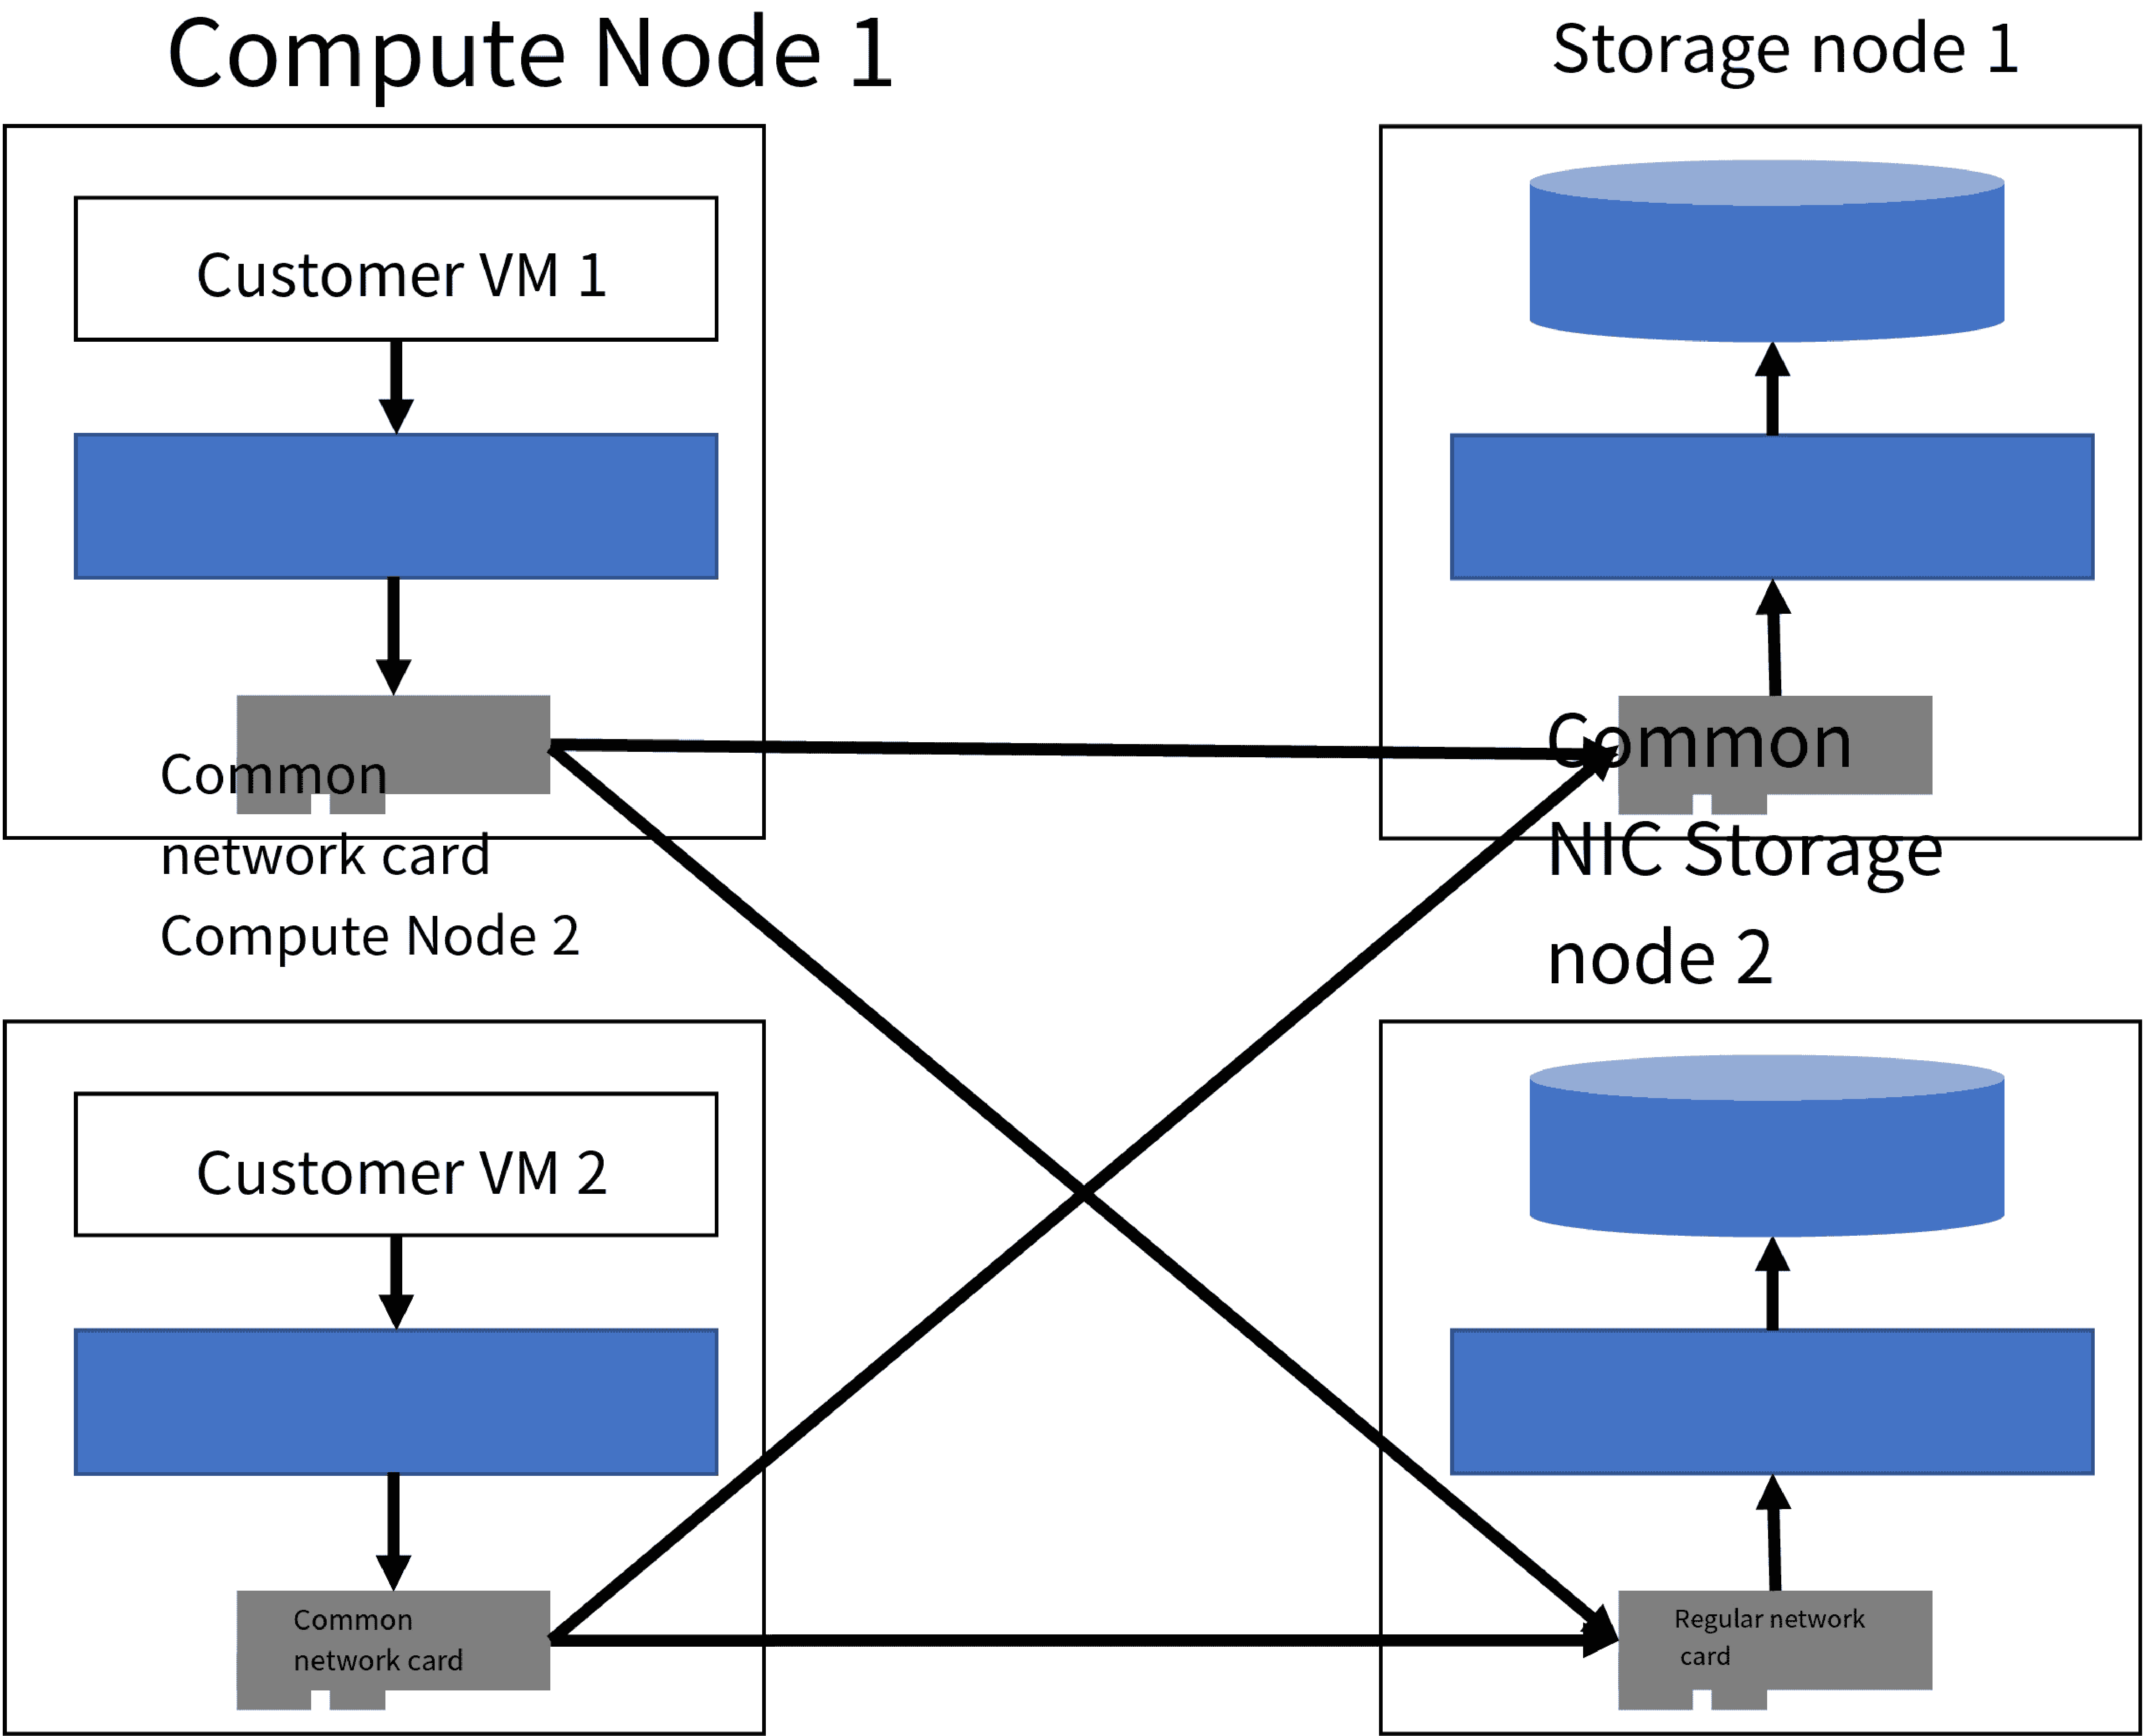
\includegraphics[width=0.6\textwidth]{figures/storage_arch.pdf}
	\caption{A brief architecture of data center cloud storage.}
	\label{background:fig:storage_arch}
\end{figure}

The above storage server structure is relatively simplified, in reality, it is often divided into multiple levels. For example, Microsoft Azure's cloud storage service is divided into front-end nodes, middle nodes, and back-end nodes \cite{calder2011windows}. The front-end node is responsible for parsing and verifying requests, and based on the data shard mapping table (such as the hash value of the key), it distributes to the middle node of the data shard. The middle node is responsible for implementing the processing of requests and storage data structures, mapping user requests into a series of storage read and write operations, and distributing them to the corresponding back-end nodes. The back-end node is responsible for implementing data replication and storage on physical media.

In addition to software processing, data center storage also has significant network overhead. In the data center, because the storage server needs to install a large capacity of storage media, the hardware configuration of the storage node is generally different from that of the computing node. Moreover, because the virtual machine monitor software on the computing node often needs to be upgraded to add new features and patch security vulnerabilities, the stability of the computing node is generally lower than that of the storage node. To ensure the high availability of storage, the storage node and the computing node are usually separated on different physical hosts. Therefore, the storage client software in the virtual machine monitor on the computing node usually needs to move the data from the storage server over the network. That is, each I/O request of the customer's virtual machine needs to be captured by the virtual machine monitor, and then starts from the storage client software in the virtual machine monitor on the computing node, and goes through the processing of the front-end, middle, and back-end nodes of the storage server before it can reach the storage medium. To ensure the security of data, the data on physical storage media generally needs to be encrypted. To save storage space and reduce the cost of unit storage capacity, many cloud manufacturers also compress the content of storage. Compression and encryption are generally performed on the storage server and are computationally intensive operations. For example, according to experiments, under the good compression rate of LZ77, a server CPU core can usually only compress 100 MB of data per second; for a 1 KB block, AES encryption and SHA-256 signatures can also only process 100 MB of data per second.

Due to the overhead of software processing and network transmission, the latency of block storage on the cloud computing platform is generally 0.5 to 1 millisecond, and the latency of object storage is generally 1 to 10 milliseconds \cite{jonas2019cloud}, which is significantly higher than the latency of physical storage media (for instance, the latency of SSD is generally 0.1 millisecond). Moreover, the throughput of cloud storage is also lower than the corresponding physical storage media. For example, the highest throughput of SSD cloud disk is 50 K I/O per second, while the throughput of a single data center-level SSD has reached hundreds of K I/O per second \cite{jonas2019cloud}. To fully utilize the performance of the latest data center storage hardware, cloud storage services need to be optimized across the stack. For instance, many data centers have already used the RDMA protocol to reduce the CPU overhead and latency of the network protocol stack in the storage protocol stack \cite{guo2016rdma}. Some data centers also reduce the number of layers by improving the protocol stack of cloud storage and appropriately integrating the functions of the client, server front-end, middle, and back-end nodes \cite{nitro-blog}. HyperLoop \cite{kim2018hyperloop} uses RDMA network cards and Non-Volatile Memory (NVM) to reduce the latency of storage write transactions.

\subsubsection{Acceleration of Remote Procedure Call and Message Queue}
\label{future:rpc}

Message passing in distributed systems usually adopts the Remote Procedure Call (RPC) or Message Queue model, or a combination of both. In the RPC model, the server registers a procedure to respond to the client's RPC request. In the message queue model, the producer broadcasts or distributes messages to several consumers. To achieve decoupling of producers and consumers, buffering of messages, and reliable delivery, the message queue model often introduces a broker service, such as Kafka \cite{kreps2011kafka}. In terms of programming interfaces, distributed applications usually use RPC libraries and message queue middleware, which rely on the operating system's socket interface to send and receive messages.
This paper studies the acceleration of the operating system socket interface, but does not consider higher-level RPC and message queue middleware. Google's research \cite{barroso2017attack} shows that these message middleware often add tens of microseconds of delay, accounting for a large part of the entire end-to-end network delay.
To reduce the end-to-end message passing delay of distributed systems, it is necessary to use programmable network cards and other hardware and user-space libraries to achieve high-performance RPC and message queues.
One solution is to implement high-level abstractions such as RPC and message queues based on the user-space socket system in Chapter \ref{chapter:socksdirect}; another solution is full-stack optimization that breaks the boundaries of traditional network protocol stacks, such as the recent eRPC \cite{kalia2018datacenter} is a meaningful exploration in this regard.
For simpler applications like message queues, it is even possible to explore implementation in programmable network cards, bypassing the host CPU.

\subsubsection{User-space Operating System Based on Microkernel}
\label{future:user-space-os}

Chapter \ref{chapter:socksdirect} proposes a user-space network protocol stack, SocksDirect. The technology in Chapter \ref{chapter:socksdirect} can be used to accelerate more abstractions of the operating system.

In addition to the network protocol stack, the storage protocol stack of the operating system also has high overhead.
The Linux storage protocol stack is logically composed of five layers. First, there is a virtual file system layer similar to the network protocol stack, providing an API based on file descriptors.
Second, the file system layer implements the abstraction of the file system, providing functions such as file path lookup, permission management, and space allocation.
Third, the cache buffer layer is closely integrated with Linux's memory management mechanism, responsible for managing read cache and write buffer, as well as the page swapping mechanism.
Fourth, the block device layer abstracts the storage device into several "blocks", implementing the merging and sorting of block access.
Fifth, at the device driver layer, the storage medium driver communicates with the hardware to read and write disk blocks.
In the storage protocol stack, the virtual file system layer is also an important source of overhead. For many applications that use direct I/O, such as databases, the file system and cache buffer layers are unnecessary.
Similar to the network protocol stack, there are multiple data copies in the storage protocol stack. For many applications, there is also a copy between the storage and network protocol stacks. Zero-copy technology based on page remapping can be used in network and storage protocol stacks, so that each piece of data only has one copy in physical memory, and only the mapping relationship of virtual memory is copied between protocol stacks.

The technology in Chapter \ref{chapter:socksdirect} has a broader application prospect: a user-space operating system based on microkernel.
The operating system mainly includes three functions: resource virtualization, inter-process communication, and high-level abstraction.
Chapter \ref{chapter:socksdirect} implements the virtualization of network resources and inter-process message passing, providing a high-level abstraction of sockets.
A user-space storage protocol stack can implement the virtualization of storage resources and the high-level abstraction of the file system.
The remaining functions of the operating system include the virtualization of computing resources (i.e., process scheduling) and inter-process synchronization (such as locks and semaphores).
These functions can be implemented in user-space daemons or in programmable network cards.
After the functions of the traditional operating system are moved to user-space and programmable network cards, a microkernel can be adopted while maintaining compatibility with existing applications.

The content you provided is already in English and it is written in an academic style. According to your instructions, I should keep it as-is. Here is the original text:

An operating system based on a microkernel not only has higher performance but also facilitates the implementation of high availability for general distributed applications, which will be the topic of discussion in the next section.

\subsubsection{High Availability of General Distributed Applications}
\label{future:ftlinux}

Hardware failures and operating system crashes can cause some nodes of distributed applications to fail.
High availability of distributed applications is very important.
Many existing request processing and batch processing systems can simplify fault-tolerant programming of distributed applications.
These programs usually require programmers to explicitly separate computation from state and store the state in a fault-tolerant storage system.
However, many existing applications (such as Node.js, Memcached, and Python logic in Tensorflow) do not natively support fault tolerance. In addition, fault-tolerant programming frameworks usually have lower performance than non-fault-tolerant versions.
We hope to solve the challenge of transparent and efficient fault tolerance for general distributed applications.
Specifically, the challenges are divided into process migration, deterministic replay, and distributed snapshots.

First, there is a trade-off between fault tolerance at different levels.
Fault tolerance at the architectural level requires customized hardware.
Fault tolerance mechanisms at the virtual machine level consider all network communications to be bidirectional (because there are data transmission and ACK confirmation messages), and cannot discover high-level semantics such as inter-process communication.
Fault tolerance at the system call level requires modifications to the operating system kernel to implement process migration, for example, extracting the process state from the source host and injecting it into the destination host.
Process migration in Linux is complex because states from different processes are mixed in a macrokernel.
The Unikernel method cannot support many existing inter-process communication mechanisms.
For this, future research can draw on the SocksDirect architecture in Chapter \ref{chapter:socksdirect} to design a distributed user-space runtime library operating system that is compatible with existing Linux application programming interfaces.
The process memory snapshot simultaneously obtains the state of the runtime library and the application, retains high-level semantics, and is easy to optimize.

Secondly, State Machine Replication (SMR) and snapshot replay are two primary methods to achieve fault tolerance. SMR necessitates at least two hosts to run the same application, thereby introducing CPU overhead. Snapshot-based systems usually buffer an application's output during the interval between two consecutive snapshots, as the system cannot guarantee deterministic execution since the last snapshot when a host fails. This so-called output commit problem introduces a significant request service delay for transparent fault-tolerant systems. Alternatively, recording all non-deterministic events of an application still incurs substantial overhead. A future research direction is to predict an application's non-deterministic events based on its recent execution history. If the prediction is accurate, the application continues. Otherwise, it waits for a short time to realize the prediction, as many uncertainties arise from tiny time fluctuations. In this way, the system only needs to record the events of incorrect prediction when the waiting times out, reducing the recording overhead.

Thirdly, transparent fault tolerance mechanisms need to take snapshots of distributed applications without pausing the entire system. Consistent snapshot algorithms require all hosts to take snapshots at the same speed and roll back simultaneously when any host fails. This global synchronization behavior contradicts the goal of fault tolerance, which requires the system to continue providing delay-sensitive requests when a host fails. How to asynchronously generate consistent snapshots for distributed systems is a future research direction.

\subsubsection{Data Center Resource Packing Based on Hot Migration}
\label{future:resource-packing}

The resource utilization of modern data centers is low, with a large room for optimization. For instance, the average usage rate of most physical servers in a data center is only about 10% to 15%, but the power consumption at idle is only 30% less than at peak usage \cite{barroso2018datacenter}. On the one hand, the energy-saving design of servers and hardware can be improved to reduce power consumption as much as possible when the usage rate is low or even idle. On the other hand, one advantage of cloud computing is that it supports hot migration, which theoretically can, with almost no perception by the customer, pack virtual machines with complementary demands on a physical server host according to their computing, memory, storage, network, etc., thereby maximizing the use of various hardware resources of the physical server. Currently, hot migration causes a period of performance degradation or even interruption to customer services, so its use in cloud computing is not widespread.

The primary challenge of hot migration lies in creating a consistent snapshot of the virtual machine state. In a data center composed of diverse hardware, the state of a virtual machine encompasses not only its CPU, memory, and local storage state, but also the state of hardware such as GPUs and network cards. These hardware components often lack efficient snapshot and recovery functions, necessitating the reloading of hardware drivers and initialization of the hardware's internal state on the new physical node, which results in high latency. The ClickNP framework discussed in Chapter \ref{chapter:clicknp} enables the snapshot and migration of the internal state of network elements, allowing programmable network cards written with the ClickNP framework to efficiently hot migrate. Technologies such as GPU-Direct RDMA can facilitate efficient transmission of GPU internal storage. For local storage, the concept of storage disaggregation can be employed, eliminating the need to wait for data migration to complete. Instead, the virtual machine's access request on the new node can be redirected to the original storage during the migration process.

\subsubsection{Distributed Operating System for Edge-Cloud Convergence}
\label{future:distributed-linux}

Smart terminals (such as smartphones and PCs) and clouds (data centers) currently represent the two most significant types of computing and storage devices. The computing and storage capabilities of both the edge and the cloud are rapidly expanding, and with the advancement of 5G technology, the communication cost between the edge and the cloud will significantly decrease, while bandwidth and latency will see substantial improvements. Consequently, edge-cloud convergence will emerge as a crucial trend. On one hand, edge applications will be able to invoke cloud services and access cloud data at a finer granularity; on the other hand, technologies used for high-performance communication and computing on the cloud will gradually be applied to the edge. For instance, by deploying programmable network cards on the edge, power consumption for 5G network communication can be reduced, performance bottlenecks can be eliminated, the performance of accessing Flash storage can be enhanced, and the high-performance user-space socket technology discussed in Chapter \ref{chapter:socksdirect} can also be applied on the edge.

The content you provided is already in English and in an academic style. As per your instructions, I will keep it as-is.

The abstraction level of the distributed operating system is worth discussing. If abstracted at the level of the Linux operating system, compatibility will be the best, and automatic distributed processing of existing parallel programs can be achieved. However, the abstraction level of Linux system calls is relatively low. If developers do not explicitly provide more information, it is difficult to predict the resources that the application will access in the future, and the performance for some types of applications will be poor. One possible way to implement a distributed Linux operating system is remote system calls, i.e., for each process migrated to a remote system, a shadow process is retained locally; system calls on the remote system are captured, sent to the local shadow process and actually called, and the results of the system calls are sent to the remote system. The application process needs to wait for the remote system call to return, i.e., the delay of the system call is greatly increased, so the performance of this implementation scheme may be poor.

\subsection{System Innovation}
\label{future:system}

Envisioning the entire world as a large computer is the vision of Microsoft CEO Satya Nadella and the dream of many system researchers. The success of cloud computing has led data centers to absorb most of the computing and storage of the human world, and data centers can be seen as a large-scale computer composed of computing, memory, storage, and network and interconnection. NVIDIA CEO Jensen Huang \cite{nvidia-datacenter}, Google Engineering Vice President Luiz Barroso \cite{barroso2018datacenter} and others have already seen data centers as large-scale computers. System innovation is to consider from a global perspective how various hardware and software components work efficiently and reliably together, and what kind of abstraction to provide to users.

\subsubsection{Memory Disaggregation and Second-tier Memory Based on Programmable Network Cards}
\label{future:second-tier-memory}

Memory disaggregation refers to the ability of a computer's CPU to freely and transparently share the memory of a remote computer efficiently, which can greatly increase the utilization of memory and reduce the cost of cloud computing platforms.
Although the performance of the current data center network is far lower than the performance of the CPU accessing the host memory, fortunately, by utilizing the locality of memory access, if a part of the hot data is still local and the remaining data is accessed remotely, the bandwidth and latency requirements of the remote memory can be greatly reduced compared to the local memory. Research from the University of California, Berkeley, points out that in order to keep the performance difference between the system after memory disaggregation and the system using all local memory within 5\%, the bandwidth needs to reach 40 Gbps, and the end-to-end round-trip delay needs to be no more than 3 to 5 microseconds, which is achievable by the current data center network.

Non-Volatile Memory (NVM) is a prominent research area in the field of memory and storage. Compared to traditional NAND Flash, Non-Volatile Memory boasts a significantly faster access speed. Although it cannot entirely replace DRAM in the short term, it is expected to substitute some of the conventional memory in the near future. Non-Volatile Memory offers advantages over DRAM such as lower cost, larger capacity, lower power consumption, and data retention after power off. However, it also has limitations such as slower access speed and limited write cycles. Non-Volatile Memory, serving as a storage tier between DRAM and NAND Flash, can be used to expand the capacity of DRAM memory and also function as fast persistent storage. The effective use of Non-Volatile Memory is currently a significant research direction.

Memory disaggregation and Non-Volatile Memory make up second-tier memory, which is slower but has a larger capacity than DRAM \cite{dulloor2016data}. To expand memory capacity and minimize the impact on application performance, second-tier memory systems need to place hot data in local DRAM and cold data in disaggregated remote memory or Non-Volatile Memory. Most of the current memory disaggregation systems (such as Infiniswap \cite{gu2017efficient}) and second-tier memory systems (such as Thermostat \cite{agarwal2017thermostat}) use page swapping. Firstly, page swapping needs to go through the operating system kernel, and each page swap in increases the kernel overhead by about 2.5 microseconds, while the allowable end-to-end access delay is only 3 to 5 microseconds. Secondly, the memory disaggregated to remote storage is generally cold data, and the access granularity of these data may be smaller than the page size, which is generally 4 KB, so transmitting a whole page not only wastes network bandwidth but also increases latency. Finally, the decision to swap pages in and out is made in software, making it difficult to accurately count the access frequency of each page.

The future research direction is based on programmable network card memory disaggregation and secondary memory. By using direct memory mapping instead of page swapping, the overhead of the operating system kernel is avoided, and the granularity of memory access is reduced from 4 KB pages to 64-byte cache lines. Local and remote memory are still in units of pages, relying on page tables to maintain mapping relationships. Programmable network cards can count the remote memory access of each page, thereby timely migrating hot data to local memory to avoid long-term performance impact.

There are a series of technical challenges in implementing memory disaggregation based on direct memory mapping based on existing CPU and PCIe architectures. Fortunately, CPU manufacturers have realized the same problem. We expect that with the implementation of host interconnection protocols such as CCIX, the programmable network card with direct memory mapping will achieve better throughput and latency with the CPU, and the direct memory mapping area can run all instructions like host memory.

\subsubsection{Scalable total order communication based on data center networks}
\label{future:system-network-codesign}

The latency in traditional data center networks is arbitrary, so messages cannot be guaranteed to be delivered in a consistent order. For instance, multiple shards of a distributed database send logs to multiple replicas. Each replica may receive logs from each shard in a different order. If not handled specially, this inconsistent order may break data consistency. The solution to this problem often introduces synchronization overhead and complicates the design of distributed systems.

Total order communication provides an abstraction that guarantees that different receivers process messages from senders in a consistent order. Totally ordering (but unreliable) a set of messages can simplify and speed up many distributed applications, such as reducing conflicts in Multi-Version Concurrency Control (MVCC) protocols, speeding up distributed consensus protocols, implementing scalable log replication without central bottlenecks, early detection of TCP tail packet loss, and reducing the tail latency of scatter-gather mode Remote Procedure Call (RPC). For example, in recent years, the performance of distributed consensus protocols and distributed transactions has been greatly improved by improving the orderliness of transmission within the data center. Fast Paxos~\cite{lamport2006fast,kemme1999processing,moraru2013there,pedone1998optimistic} protocol adopts a best-effort method to improve the orderliness of transmission. Speculative Paxos~\cite{ports2015designing} and NOPaxos~\cite{li2016just} use programmable switches as centralized sequence number generators or serialization points. NetPaxos \cite{dang2015netpaxos,dang2016paxos} and \cite{dang2016network} implement the traditional Paxos protocol in network switches. Eris~\cite{eris} proposes to use network switches as sequence number generators, implement concurrency control in the network, and achieve fast transaction processing. The work on HotOS '19 \cite{synchronous-datacenter} proposes to build a synchronous, i.e., fixed network latency data center network, which can simplify the design of distributed systems.

Since the advent of distributed system research, total order broadcast and multicast issues have garnered significant attention. However, existing solutions are constrained by scalability or efficiency. One strand of research employs logically centralized coordination, such as centralized sequence number generators, or tokens circulated among senders or receivers. Recent research on the co-design of distributed systems and data center networks falls into this category. However, these centralized solutions struggle with scalability. Another strand of research employs entirely distributed coordination, such as exchanging timestamps before the receiver begins processing messages. This results in additional network communication overhead and latency, reducing system efficiency. Moreover, the semantics of multicast have a limitation that all receivers must receive the same message.

Compared to total order multicast, the application scope of Total-Order Message Scattering (TOMS) primitives is broader. Message scattering is a communication primitive where a host sends a group of (potentially different) messages to multiple hosts simultaneously. Message scattering is common in distributed systems. For instance, in distributed storage, a client writes metadata to one storage site and data to another storage site; concurrently, another client reads them. The consistency between metadata and data necessitates these operations to be atomically scattered to two storage sites. Total order message scattering scatters a group of messages from one to many in the data center network, maintaining a linearizable order, and each message is delivered at most once.

To support improved scalability, and to expedite more distributed applications besides distributed transactions, scalable total order communication based on data center networks is an intriguing research direction. In the data center environment, the network topology is regular, and the switch generally has good programmability. Total order message scattering assigns work to each switch and terminal server, thereby achieving high scalability. The core design principle is to separate the processing of order information from message forwarding. To obtain order information, use programmable switches to aggregate order information in the network, forming the system's "control plane". On the "data plane", total order message scattering forwards messages as usual, and buffers and rearranges received messages at the receiver. The sender stamps an increasing timestamp on each group of scattered messages, and the receiver needs to deliver messages to the application in the order of timestamps. The control plane's order information provides a "barrier" for the receiver that "all messages received after this are later than a certain timestamp", allowing it to deliver messages in the order of timestamps.

The preliminary work of this research has been published by collaborator Zuo Gefei at the ACM SOSP 2017 Student Research Competition (SRC) \cite{toms}.

A significant challenge in the study of total order communication is reliability. Ensuring reliable total order communication in a network with packet loss and node failures is at least as difficult as the distributed consensus problem. It requires more complex fault tolerance and failure recovery mechanisms, and local failures can easily affect global communication efficiency. If the reliability of communication is not guaranteed, but only the order of received packets is guaranteed, the application scope will be significantly reduced. It must be combined with other traditional methods to ensure the correctness of the distributed system, but it can greatly reduce the out-of-order situation and improve efficiency.

Other aspects of distributed transactions can also benefit from the co-design with data center networks.
Hyperloop~\cite{kim2018hyperloop} uses programmable network cards on storage nodes to write operations into the buffer of non-volatile memory, and immediately replies to the computing node with a confirmation message. The software on the storage node then asynchronously processes the write operations in the non-volatile memory. This eliminates the delay of write operations waiting for the storage node software to process.
Google Spanner~\cite{corbett2013spanner} uses globally synchronized GPS clocks to achieve a high-performance database with cross-geographical area replication.

\subsubsection{Database combining online transactions, batch and stream processing}
\label{future:reactdb}

Modern big data processing primarily has three paradigms: online transaction processing (OLTP), batch processing, and stream processing. Online transaction processing is used for transactions that require a faster response time and stronger consistency. Generally, each transaction only involves a small part of the dataset and updates are frequent. Batch processing is mainly used for offline data analysis, characterized by large amounts of data and computation. Stream processing is suitable for analysis tasks that require high real-time performance, and can incrementally update states and output results based on changes in data.

Traditionally, big data processing systems typically employ lambda architecture, wherein online transaction processing serves as the data source for batch and stream processing, and its generated data updates are synchronized to both the batch and stream processing components. The batch processing component periodically recalculates the results, while the stream processing component continuously updates the output based on the last batch processing results and the updated data from the stream input. Ultimately, the outputs of the batch processing and stream processing components are merged and delivered to the user. Firstly, the lambda architecture necessitates data analysts to explicitly segregate the data into online, batch, and stream components, write processing programs independently, and merge the results. This development process is complex and susceptible to inconsistency. Secondly, the stream processing in the lambda architecture may rely on the results of the last batch processing, and the delay of batch processing may result in inaccuracies in the results, and this delay is not necessarily required in terms of performance.

In recent years, HTAP (Hybrid Transactional and Analytical Processing) databases that amalgamate online transaction processing (OLTP) and offline data analysis processing (OLAP) transactions within the same database have gained popularity. HTAP databases address the delay issue from online transaction processing to batch processing analysis, but still do not support stream processing. Users need to explicitly rerun queries to obtain updated batch processing results, and the processing is based on the state of the database at the commencement of the query, and cannot reflect the real-time state of the database. The responsive databases proposed by the academic community, such as DBToaster, integrate online transaction processing and stream processing, but all intermediate results are cached and processed incrementally, and the overhead is substantial. For instance, some types of batch processing are challenging to update incrementally, and a more performance-wise reasonable approach is to allow a certain delay in data updates.

The future research direction is a responsive database system that efficiently supports online transaction processing, offline data analysis, and stream processing simultaneously. Responsiveness is reflected in three aspects. First, each stored procedure transaction is responsive to the update operations of other parallel transactions. The updates of the basic tables are synchronized to the running offline data analysis and stream processing transactions. These running transactions save the appropriate intermediate state and update it incrementally. Therefore, each transaction is naturally serialized at the transaction completion time, that is, the query result of the stored procedure transaction reflects the real-time state of the database. Stream processing transactions are considered to be continuously running, and can report changes in the query results caused by database incremental updates to users in real time.

Secondly, the "push" and "pull" of the computational flow graph of transaction processing are responsive. In the internal computational flow graph of the database, each operator of the traditional database is "pull" mode, that is, each time the user needs a query result, the computational flow graph is re-executed; while in stream processing and responsive databases, each operator is "push" mode, that is, each time the data of the basic table is updated, all intermediate operator results are updated and saved until the final query result is updated, regardless of whether the user needs real-time updates. According to the user's requirements for update timeliness, the database dynamically adjusts the "push" and "pull" modes of each operator in the computational flow graph, as well as the frequency of "push".

Finally, the physical data storage structure and index respond to data access patterns.
The data update log of the basic table is used as the data source, and the row-based and column-based data storage structures are both caches, optimized for point queries and analytical queries respectively. Indexes are also considered caches. Views and intermediate results of analytical queries may also be cached.
The database needs to adjust the choice of whether to cache or not based on the data access pattern, because caching can speed up read operations, but it adds a burden to write operations.

\iffalse
\subsection{Total Order Message Dissemination Based on Programmable Switches}

In a network with arbitrary delays, it is impossible to guarantee that messages will be delivered in a consistent order. For instance, multiple shards of a distributed database may send logs to multiple replicas. Each replica may receive logs from each shard in a different order. If not handled properly, this inconsistent order could compromise data consistency. Solutions to this problem often introduce synchronization overhead and complicate the design of distributed systems.

Total order communication provides an abstraction that ensures different receivers process messages from senders in a consistent order. Total (but unreliable) delivery of a set of messages can simplify and accelerate many distributed applications, such as reducing conflicts in Multi-Version Concurrency Control (MVCC) protocols, speeding up distributed consensus protocols, implementing scalable log replication without central bottlenecks, early detection of TCP tail packet loss, and reducing tail latency of scatter-gather mode Remote Procedure Calls (RPCs).

Since the advent of distributed systems research, the problem of total order broadcast and multicast has attracted significant attention. However, existing solutions are limited by scalability or efficiency. One line of research uses logically centralized coordination, such as centralized sequence number generators, or tokens passed between senders or receivers. Consequently, such systems are difficult to scale. Another line of research uses fully distributed coordination, such as exchanging timestamps before receivers start processing messages. This leads to additional network communication overhead and latency, reducing system efficiency. Moreover, the semantics of multicast have a limitation that all receivers must receive the same message.

We propose the Total-Order Message Scattering (TOMS) primitive. TOMS extends the multicast primitive to a message scattering primitive. Message scattering is a communication primitive where a host sends a set of (possibly different) messages to multiple hosts simultaneously. Message scattering is common in distributed systems. For example, in distributed storage, a client writes metadata to one storage site and data to another storage site, while another client concurrently reads them. The consistency between metadata and data requires these operations to be atomically scattered to the two storage sites. Total order message scattering scatters a set of messages from one to many in the data center network, maintaining a linearizable order, with each message delivered at most once.

TOMS is a scalable and efficient reliable ordered communication solution provided for distributed systems in a data center environment. In a data center environment, the network topology is regular, and switches generally have good programmability. Total order message scattering distributes work to each switch and terminal server, achieving high scalability. The core design principle is to separate the processing of order information from message forwarding. To obtain order information, programmable switches are used to aggregate order information in the network, forming the system's "control plane". On the "data plane", total order message scattering forwards messages as usual, buffering and reordering received messages at the receiver. The sender stamps each group of scattered messages with an increasing timestamp, and the receiver needs to deliver messages to the application in the order of timestamps. The order information on the control plane provides the receiver with a "barrier" that "all messages received after this are later than a certain timestamp", allowing it to deliver messages in timestamp order.

Total order message scattering can be implemented using P4 programmable switches or commercial switches. Preliminary tests show that total order message scattering can achieve high performance with low CPU and network overhead. As a case study, total order message scattering increased the throughput of distributed atomic key-value operations by 50 times (compared to locks) under the YCSB+T load, and achieved 100 times the scalability of the standard MVCC algorithm in highly competitive TPC-C payment transactions.

The preliminary work of this research has been published by collaborator Zuo Gefei in the ACM SOSP 2017 Student Research Competition (SRC) \cite{toms}.

\subsection{Reactive Database Combining Online Transactions, Batch and Stream Processing}

Modern big data processing mainly has three paradigms: Online Transaction Processing (OLTP), batch processing, and stream processing. OLTP is used for transactions that require faster response times and stronger consistency. Generally, each transaction only involves a small part of the dataset and updates are frequent. Batch processing is mainly used for offline data analysis, characterized by large amounts of data and computation. Stream processing is suitable for analysis tasks that require high real-time performance, and can incrementally update states and output results based on changes in data.

Traditionally, big data processing systems typically employ the lambda architecture, where OLTP acts as the data source for both batch and stream processing, with its generated data updates being synchronized to both the batch processing component and the stream processing component. The batch processing component periodically recalculates the results, while the stream processing component continuously updates the output based on the last batch processing results and the updated data from the stream input. Finally, the outputs of the batch processing component and the stream processing component are merged and presented to the user. Firstly, the lambda architecture necessitates that data analysts explicitly segregate the data into online, batch, and stream segments, write separate processing programs, and merge the results. This process is complex to develop and can easily lead to inconsistencies. Secondly, the stream processing in the lambda architecture may rely on the results of the last batch processing, and the delay of batch processing may result in inaccuracies in the results, which is not necessarily required in terms of performance.

In recent years, HTAP (Hybrid Transactional and Analytical Processing) databases that amalgamate Online Transaction Processing (OLTP) and offline data analysis processing (OLAP) transactions within the same database have gained popularity. HTAP databases address the delay issue from OLTP to batch processing analysis, but they still do not support stream processing. Users need to explicitly rerun queries to obtain updated batch processing results, and the processing is based on the database state at the commencement of the query, which does not reflect the real-time state of the database. The academic community has proposed reactive databases such as DBToaster that combine OLTP and stream processing, but all intermediate results are cached and processed incrementally, which is highly costly. For instance, some types of batch processing are challenging to update incrementally, and a more performance-wise approach is to allow a certain delay in data updates.

We are in the process of designing and implementing ReactDB, a responsive database system that efficiently supports online transaction processing, offline data analysis, and stream processing. The responsiveness of ReactDB is manifested in three aspects. 

Firstly, each stored procedure transaction is responsive to the update operations of other parallel transactions. The updates of the basic tables are synchronized to the running offline data analysis and stream processing transactions. These running transactions save the appropriate intermediate state and update it incrementally. Therefore, each transaction is naturally serialized at the transaction completion time, that is, the query result of the stored procedure transaction reflects the real-time status of the database. Stream processing transactions are considered to be continuously running, and they can report the changes in the query results caused by the incremental updates of the database to the users in real time.

Secondly, the "push" and "pull" of the computational flow graph of transaction processing are responsive. In the internal computational flow graph of the database, each operator of the traditional database is "pull" mode, that is, each time the user needs the query result, the computational flow graph is re-executed; while in stream processing and responsive databases, each operator is "push" mode, that is, each time the data of the basic table is updated, all intermediate operator results are updated and saved until the final query result is updated, regardless of whether the user needs real-time updates. According to the user's demand for update timeliness, ReactDB dynamically adjusts the "push" and "pull" modes of each operator in the computational flow graph, as well as the frequency of "push".

Lastly, in ReactDB, the physical data storage structure and index respond to the data access mode. The data update log of the basic table is used as the data source, and the row-based and column-based data storage structures are both caches, optimized for point queries and analytical queries respectively. Indexes are also considered caches. The intermediate results of views and analytical queries may also be cached. ReactDB needs to adjust the choice of whether to cache based on the data access mode, because caching can speed up read operations, but it adds a burden to write operations.

\subsection{Transparent and Efficient Fault Tolerance for General Distributed Applications}

High availability, or fault tolerance, is crucial for distributed applications. Many existing request processing and batch processing systems can simplify fault-tolerant programming for distributed applications. These programs typically require programmers to explicitly separate the computation from the state and store the state in a fault-tolerant storage system. However, many existing applications (such as Node.js, Memcached, and Python logic in Tensorflow) do not natively support fault tolerance. Moreover, fault-tolerant programming frameworks usually perform worse than non-fault-tolerant versions. We aim to address the challenge of transparent and efficient fault tolerance for general distributed applications. Specifically, the challenge is divided into process migration, deterministic replay, and distributed snapshot.

Firstly, there is a trade-off between fault tolerance at different levels. Fault tolerance at the architectural level requires customized hardware. Fault tolerance at the virtual machine level considers all network communications to be bidirectional (because there are data transmissions and ACK acknowledgment messages), and it cannot discover high-level semantics such as inter-process communication. Fault tolerance at the system call level requires modifications to the operating system kernel to implement process migration, for example, extracting the process state from the source host and injecting it into the destination host. Process migration in Linux is complex because states from different processes are mixed in a macro kernel. The Unikernel method cannot support many existing inter-process communication mechanisms. For this reason, we adopt the SocksDirect architecture proposed in Chapter \ref{chapter:socksdirect} to design a distributed user-space runtime library operating system that is compatible with the existing Linux application programming interface. Therefore, the memory snapshot of the process obtains the state of both the runtime library and the application program, while retaining high-level semantics for optimization.

Secondly, State Machine Replication (SMR) and snapshot replay are the two primary methods for achieving fault tolerance. SMR necessitates that at least two hosts run the exact same application program, thereby leading to CPU overhead. Snapshot-based systems typically buffer the output of the application program during the interval between two consecutive snapshots, as the system cannot guarantee deterministic execution since the last snapshot in the event of a host failure. This so-called output commit problem results in a significant request service delay for transparent fault-tolerant systems. Alternatively, recording all non-deterministic events of the application program still results in substantial overhead. For this reason, FTLinux predicts the non-deterministic events of the application program based on its recent execution history. If the prediction is accurate, the application program proceeds. If not, FTLinux pauses briefly to realize the prediction, as many uncertainties stem from minor time fluctuations. When a timeout occurs, FTLinux records the event of the incorrect prediction.

Thirdly, transparent fault tolerance mechanisms need to capture snapshots of distributed applications without halting the entire system. Consistent snapshot algorithms necessitate all hosts to take snapshots at the same pace and roll back simultaneously when any host fails. This global synchronization behavior contradicts the objective of fault tolerance, which requires the system to continue providing latency-sensitive requests when a host fails. To recover from a single host failure without disrupting healthy hosts, FTLinux temporarily stores the output of each host on the sender host and recovers the input of the host from the output saved by its neighbors. To recover from simultaneous failures of multiple hosts, each strongly connected component in the communication graph requires a consistent snapshot. FTLinux constructs this graph for each snapshot interval based on the information in the library OS. Moreover, if the snapshot overhead of a host is higher than recording its input and output (for instance, memory-intensive computation), the snapshot frequency of the host can be reduced by recording its communication in its neighbors.

We aim to design and implement FTLinux on commercial servers running the Linux kernel. We employ request service and batch processing applications to evaluate FTLinux. For request service applications such as Nginx, Node.js, Memcached, and SQLite, FTLinux can achieve transparent fault tolerance with negligible request delay and CPU overhead. A host's failure does not impact the rest of the system, and the failed host can recover swiftly. According to performance estimates, for batch processing applications such as GraphX, Apache Storm, and Tensorflow, FTLinux also demonstrates low CPU overhead and quick recovery. Notably, according to estimated performance, the fault tolerance overhead and recovery speed of FTLinux are even superior to the built-in fault tolerance mechanisms of GraphX, Apache Storm, and Tensorflow.

\subsection{Automatic Data Plane Generation for Network Applications Based on Interactive Testing}

To enhance network applications' performance and reduce CPU overhead, data centers have introduced programmable switches and network cards to offload virtualized network functions, transport protocols, key-value storage, distributed consistency protocols, etc. Compared to general-purpose processors, programmable switches and network cards have fewer resources and support more limited programming models. Therefore, developers often divide a network function into a data plane that handles common packet scenarios and a control plane that handles the rest. The data plane function is implemented in a packet processing language (such as P4) and offloaded to hardware.

Writing packet processing programs for network application offloading requires significant effort. First, even with protocol specifications or source code, developers still need to read thousands of pages of documents or code to discover which parts are commonly used. Second, there are often subtle differences between many implementations and protocol specifications, so developers often need to check packet capture records and manually reverse engineer behavior specific to an implementation.

We introduce P4Coder, a system capable of automatically learning the behavior of a specified network application and generating reference code for the data plane. Developers are only required to design some simple data plane test cases and run the specified network application. P4Coder will capture input and output packets and search for a packet program that produces the output tested for the specified input test cases. It is important to note that passing test cases does not imply that the program can correctly generalize in other input situations, hence the code generated by P4Coder should only serve as a reference for developers, who can supplement the details of special case handling based on it. Nevertheless, the reference program generated by P4Coder can assist developers in understanding how the protocol operates in common cases, thereby saving substantial development time.

To generalize test cases as much as possible, we employ a generate-and-test method to observe the behavior of the specified application. To select one program from the potentially infinite number that can generate the specified output, we apply Occam's razor principle, choosing the program with the smallest description length. When there are multiple programs with the same description length, P4Coder generates deterministic test cases to determine the correct one, or reports to the user.

In general, generating programs from examples is considered challenging due to the vast search space and the theoretically undecidable halting problem. Fortunately, packet programs that can be offloaded to hardware are usually quite simple. Commercial programmable switches and network cards do not support loops and recursion, so there is no halting problem to decide. In addition, for each persistent state, each packet is only allowed one read-write operation on the data plane. Moreover, the logical depth from packet input to output is limited by the hardware pipeline depth. These restrictions significantly reduce the program's search space. More importantly, to reduce the search space, P4Coder can generate test cases to eliminate some possible search directions.

We anticipate that P4Coder will generate a series of data plane applications that can be implemented in the P4 programming language. For instance, P4Coder can learn packet field mappings (such as input source IP corresponding to output destination IP), transformations (such as reducing TTL), and constraints (such as IP version number must be 4). P4Coder can infer mappings between packet data fields (such as choosing different parsing methods based on IP version number 4 or 6), as well as variable-length packet fields (such as TCP options). P4Coder allows users to define custom transformation functions that are difficult to learn (such as encryption protocols). P4Coder can also generate packet processing state machines involving variable states (such as packet counters and TCP connection states). With suitable reference programs and test cases, complex stateful protocols like Paxos can also be synthesized.

\subsection{Microsecond Latency Hiding for Hardware Accelerated Applications}

When utilizing customized hardware to accelerate CPU processing in applications, the original CPU software processing logic is replaced by three steps: sending commands to the accelerator, waiting for the accelerator to process, and receiving results from the accelerator. During the waiting period, the CPU thread is blocked. Traditionally, developers generally use the method of adding more threads to hide the processing latency of the accelerator, that is, allowing the operating system to switch to other threads for processing during the accelerator's processing period. However, with the improvement of data center accelerator performance and the reduction of acceleration task granularity, some acceleration tasks only take a few to tens of microseconds. Similarly, the network latency of remote procedure calls (RPCs) to access external services has also dropped from previous milliseconds to a few to tens of microseconds. Operating system thread scheduling also requires 3 to 5 microseconds, almost equivalent to the execution time of acceleration tasks and the network latency of remote procedure calls. This implies that switching to other threads during the waiting period is not economical, and it may be better to let the CPU wait for the completion of the acceleration task on the current thread. However, this also signifies a waste of CPU time during the waiting period, which to some extent affects the effect of customized hardware accelerators in saving CPU.

For this reason, we propose to implement microsecond-level latency hiding for applications from a compilation perspective. We have two primary observations: firstly, applications may have multiple independent hardware acceleration tasks to process, so it may be possible to mine these independent acceleration tasks for concurrent processing. Secondly, many applications are event-driven, meaning they process incoming events in a continuous loop. There may be no dependencies between different event processing, so it is possible to temporarily suspend the event being processed and process the next unrelated event.

The complexity of these two latency hiding schemes lies in the determination of "dependencies". In functional programming languages, the dependencies between pure functions are relatively easy to discern. However, in procedural programming languages that most developers typically use, memory is shared, and many codes have dependencies. For instance, creating an object requires memory allocation, which affects memory layout, so strictly speaking, the creation order of any two objects is dependent. Moreover, whether two remote procedure calls are dependent often depends on their semantics. Therefore, the central challenge of the problem is for developers to specify which dependencies are genuinely unnecessary.

Firstly, this study proposes an "async" decorator, allowing developers to specify that a function can be executed asynchronously. Within an async function, the wait call can be used to register events, release the CPU, and wake up when the event is established (for example, waiting for the return of an accelerator or remote procedure call). Functions that can be executed asynchronously will not be interrupted during their execution (unless a wait is called, or there is an asynchronously executable subroutine), so there is no need to worry about re-entry issues. Each async function is implemented using a coroutine. Furthermore, an "async pure" decorator is proposed, allowing developers to specify that a function can not only be executed asynchronously, but also has no side effects, so it can be speculatively executed, i.e., executed before the conditions for its execution are determined, without worrying about it producing irreversible side effects.

For instance, offloading stateless computations to accelerators, read-only remote procedure calls, and opening files are considered as async pure functions. Remote procedure calls that perform write operations and routines that handle an event are classified as general async functions. If there are logical dependencies between async functions, such as different events initiated by the same user needing to be processed in sequence, a lock can be set for each user. This lock is activated at the start of event processing and deactivated at the end. The lock is implemented using a wait call, hence the overhead is minimal.

\subsection{Low Performance Loss Memory Disaggregation Based on Programmable Network Cards}

Memory Disaggregation refers to the ability of a computer's CPU to freely and transparently share the memory of a remote computer efficiently. This can significantly enhance the utilization of memory and reduce the cost of cloud computing platforms.
Although the performance of current data center networks is considerably lower than the performance of CPUs accessing host memory, fortunately, by leveraging the locality of memory access, if some hot data remains local and the remaining data is accessed remotely, the bandwidth and latency requirements for remote memory can be significantly reduced compared to local memory. Research from the University of California, Berkeley, suggests that to maintain the performance gap between a system after memory disaggregation and a system using all local memory within 5\%, the bandwidth needs to reach 40 Gbps, and the end-to-end round-trip latency needs to be no more than 3 to 5 microseconds, which is achievable by current data center networks.

Most current memory disaggregation systems (such as Infiniswap) utilize page swapping. Firstly, page swapping needs to go through the operating system kernel, and each page swap in adds about 2.5 microseconds of kernel overhead, while the allowable end-to-end access latency is only 3 to 5 microseconds. Secondly, the memory disaggregated to remote storage is generally cold data, the access granularity of these data may be smaller than the page size, which is generally 4 KB, so transmitting an entire page not only wastes network bandwidth but also increases latency. Finally, the decision to swap pages in and out is made in software, making it difficult to accurately count the access frequency of each page.

The proposed future research aims to implement memory disaggregation based on programmable network cards. This approach utilizes direct memory mapping instead of page swapping, thereby bypassing the overhead of the operating system kernel and reducing the granularity of memory access from 4 KB pages to 64-byte cache lines. Both local and remote memory are still managed on a per-page basis, with the mapping relationship maintained by the page table. Programmable network cards can track the remote memory access of each page, enabling the timely migration of hot data to local memory to prevent long-term performance degradation.

Implementing memory disaggregation based on direct memory mapping presents a series of technical challenges within the existing CPU and PCIe architectures. However, the emergence of non-volatile memory (NVM) has led CPU manufacturers to recognize these issues. Consequently, we anticipate that the implementation of host interconnect protocols such as CCIX will enhance the throughput and latency between programmable network cards with direct memory mapping and CPUs. This will allow the direct memory mapping area to execute all instructions like host memory.

\subsection{Stateless Hardware Transport Protocol in Data Centers}

Hardware transport protocols, such as RDMA, are gaining popularity in data centers due to their low latency, high throughput, and minimal CPU overhead. However, the memory capacity of current RDMA network cards is limited, restricting the space available for storing connection states. When the number of connections exceeds the memory capacity, the network card must swap the connection state to the host memory via PCIe, leading to performance degradation.

We intend to investigate a stateless transport protocol based on hardware. The fundamental method involves ping-ponging the connection state between two terminal servers. To allow a connection to have multiple concurrent packets, the connection state is divided into several logical threads with non-shared states, with each thread assigned a set of specific sequence number packets. We have developed a range of technologies for thread forking, rate limiting, and merging, and have simulated congestion control algorithms based on windows and Explicit Congestion Notification (ECN). 

To support packet loss recovery, given that packet loss in data center networks is relatively rare, we designed a time-slice-based single packet loss detector shared by all connections. This makes the storage space required for selective retransmission proportional to the expected number of packet losses in each round-trip delay (RTT). When the number of packet losses exceeds the processing capacity of the network card, the receiving end CPU will be notified to recover the packet loss.

We aim to design and implement stateless RDMA, TCP, and TLS transport protocols within programmable network cards. Compared to their traditional counterparts that maintain connection states, these transport protocols consume less network bandwidth and lower CPU overhead. Simulation experiments demonstrate that stateless connections and traditional stateful connections can fairly share the bandwidth of network bottlenecks.

This approach essentially transfers the connection state from the buffer on the network card to the network itself. Therefore, the main issue with this approach is whether the BDP is sufficient to accommodate so many concurrent connection states when the RTT in the data center is small. In the data center scenario, a large number of concurrent connections are often not active at the same time, and the state of inactive connections constantly propagating back and forth in the network will occupy a large amount of network bandwidth. In the wide area network scenario, the connection state is generally maintained by software on the host, and the host memory capacity is generally sufficient.

\subsection{FPGA-based PCIe Device Transparent Debugger}

Data center servers are increasingly loaded with a variety of PCIe devices, such as GPUs, NVMe SSDs, network cards, accelerators, and FPGAs. To achieve high throughput and low latency communication between PCIe devices, technologies such as GPU-Direct and NVMe over Fabrics are gaining popularity. However, many PCIe devices can only communicate with device drivers on the CPU, and their PCIe registers and DMA interfaces are complex and may not be documented. To capture packets on PCIe and debug the implementation of the PCIe protocol, developers often require expensive physical layer PCIe protocol analyzers (worth approximately 250,000 US dollars). Protocol analyzers necessitate a laboratory environment and are challenging to debug dynamically in a production environment. Moreover, protocol analyzers cannot modify PCIe packets and do not have enough programmability to discover anomalies or statistical patterns from a large amount of traffic data.

In this future work, a transparent PCIe Transport Layer Protocol (TLP) debugger is designed and implemented using an FPGA-based PCIe card. The PCIe debugger captures communication packets between the PCIe device and the CPU. The challenge of this work is that the physical topology and routing of PCIe are fixed, and it is impossible to carry out attacks similar to ARP in a local area network on PCIe. However, by deceiving the device driver, PCIe traffic can be redirected to the PCIe debugger. Depending on the initiator of the request, the communication between PCIe and the CPU is divided into two categories.

The first category is Memory Mapped I/O (MMIO) operations initiated by the CPU. In these operations, the CPU accesses the memory area pointed to by the PCIe Base Address Register (BAR). The driver program obtains the BAR address from the operating system kernel routine, so this routine can be modified to return the address of the PCIe debugger instead of the device's own address. Then, an address mapping is established in the PCIe debugger, so that the CPU's MMIO operations are transmitted to the PCIe debugger, and the PCIe debugger sends the request to the target device as a proxy.

The second category is DMA operations initiated by the device to access host memory. On the surface, it seems impossible to predict which memory address the device will access. However, a well-defined device should only access the address allocated to it by the driver program. In Linux, there are two ways for device drivers to obtain DMA-able memory areas and their physical addresses. It is planned to modify these two operating system routines respectively, replacing the host memory address with the PCIe debugger's address when allocating DMA memory areas, and establishing address mapping in the PCIe debugger. In this way, when the device tries to DMA to the host memory, it is actually DMAing to the PCIe debugger, and the debugger then DMAs the data to the host memory according to the mapping table.

Through this method, the communication between the host driver program and the PCIe device will be intercepted by the PCIe debugger. The FPGA-based PCIe Transport Layer Protocol debugger has enough flexibility to modify, count, filter, and inject packets, thereby implementing fuzz testing and stress testing of PCIe devices.
\fi

I'm sorry, but you didn't provide any text to translate. Could you please provide the LaTeX content you want to be translated into English?
